\begin{textblock*}{\paperwidth}(0cm, 0pt)%
    \noindent\makebox[\paperwidth][l]{\includegraphics[height=\paperheight]{utilities/configuration_ultra.jpg}}%
\end{textblock*}%

\begin{textblock*}{13.4cm}(.5cm, 8cm)%
    \noindent%
    \begin{tikzpicture}%
        \fill[white, opacity=0.88] (0,0) rectangle (13.8cm,5.0cm);%
    \end{tikzpicture}%
\end{textblock*}%

\begin{sffamily}%
    \begin{textblock*}{4cm}(1.0cm, 8.5cm)%
        \noindent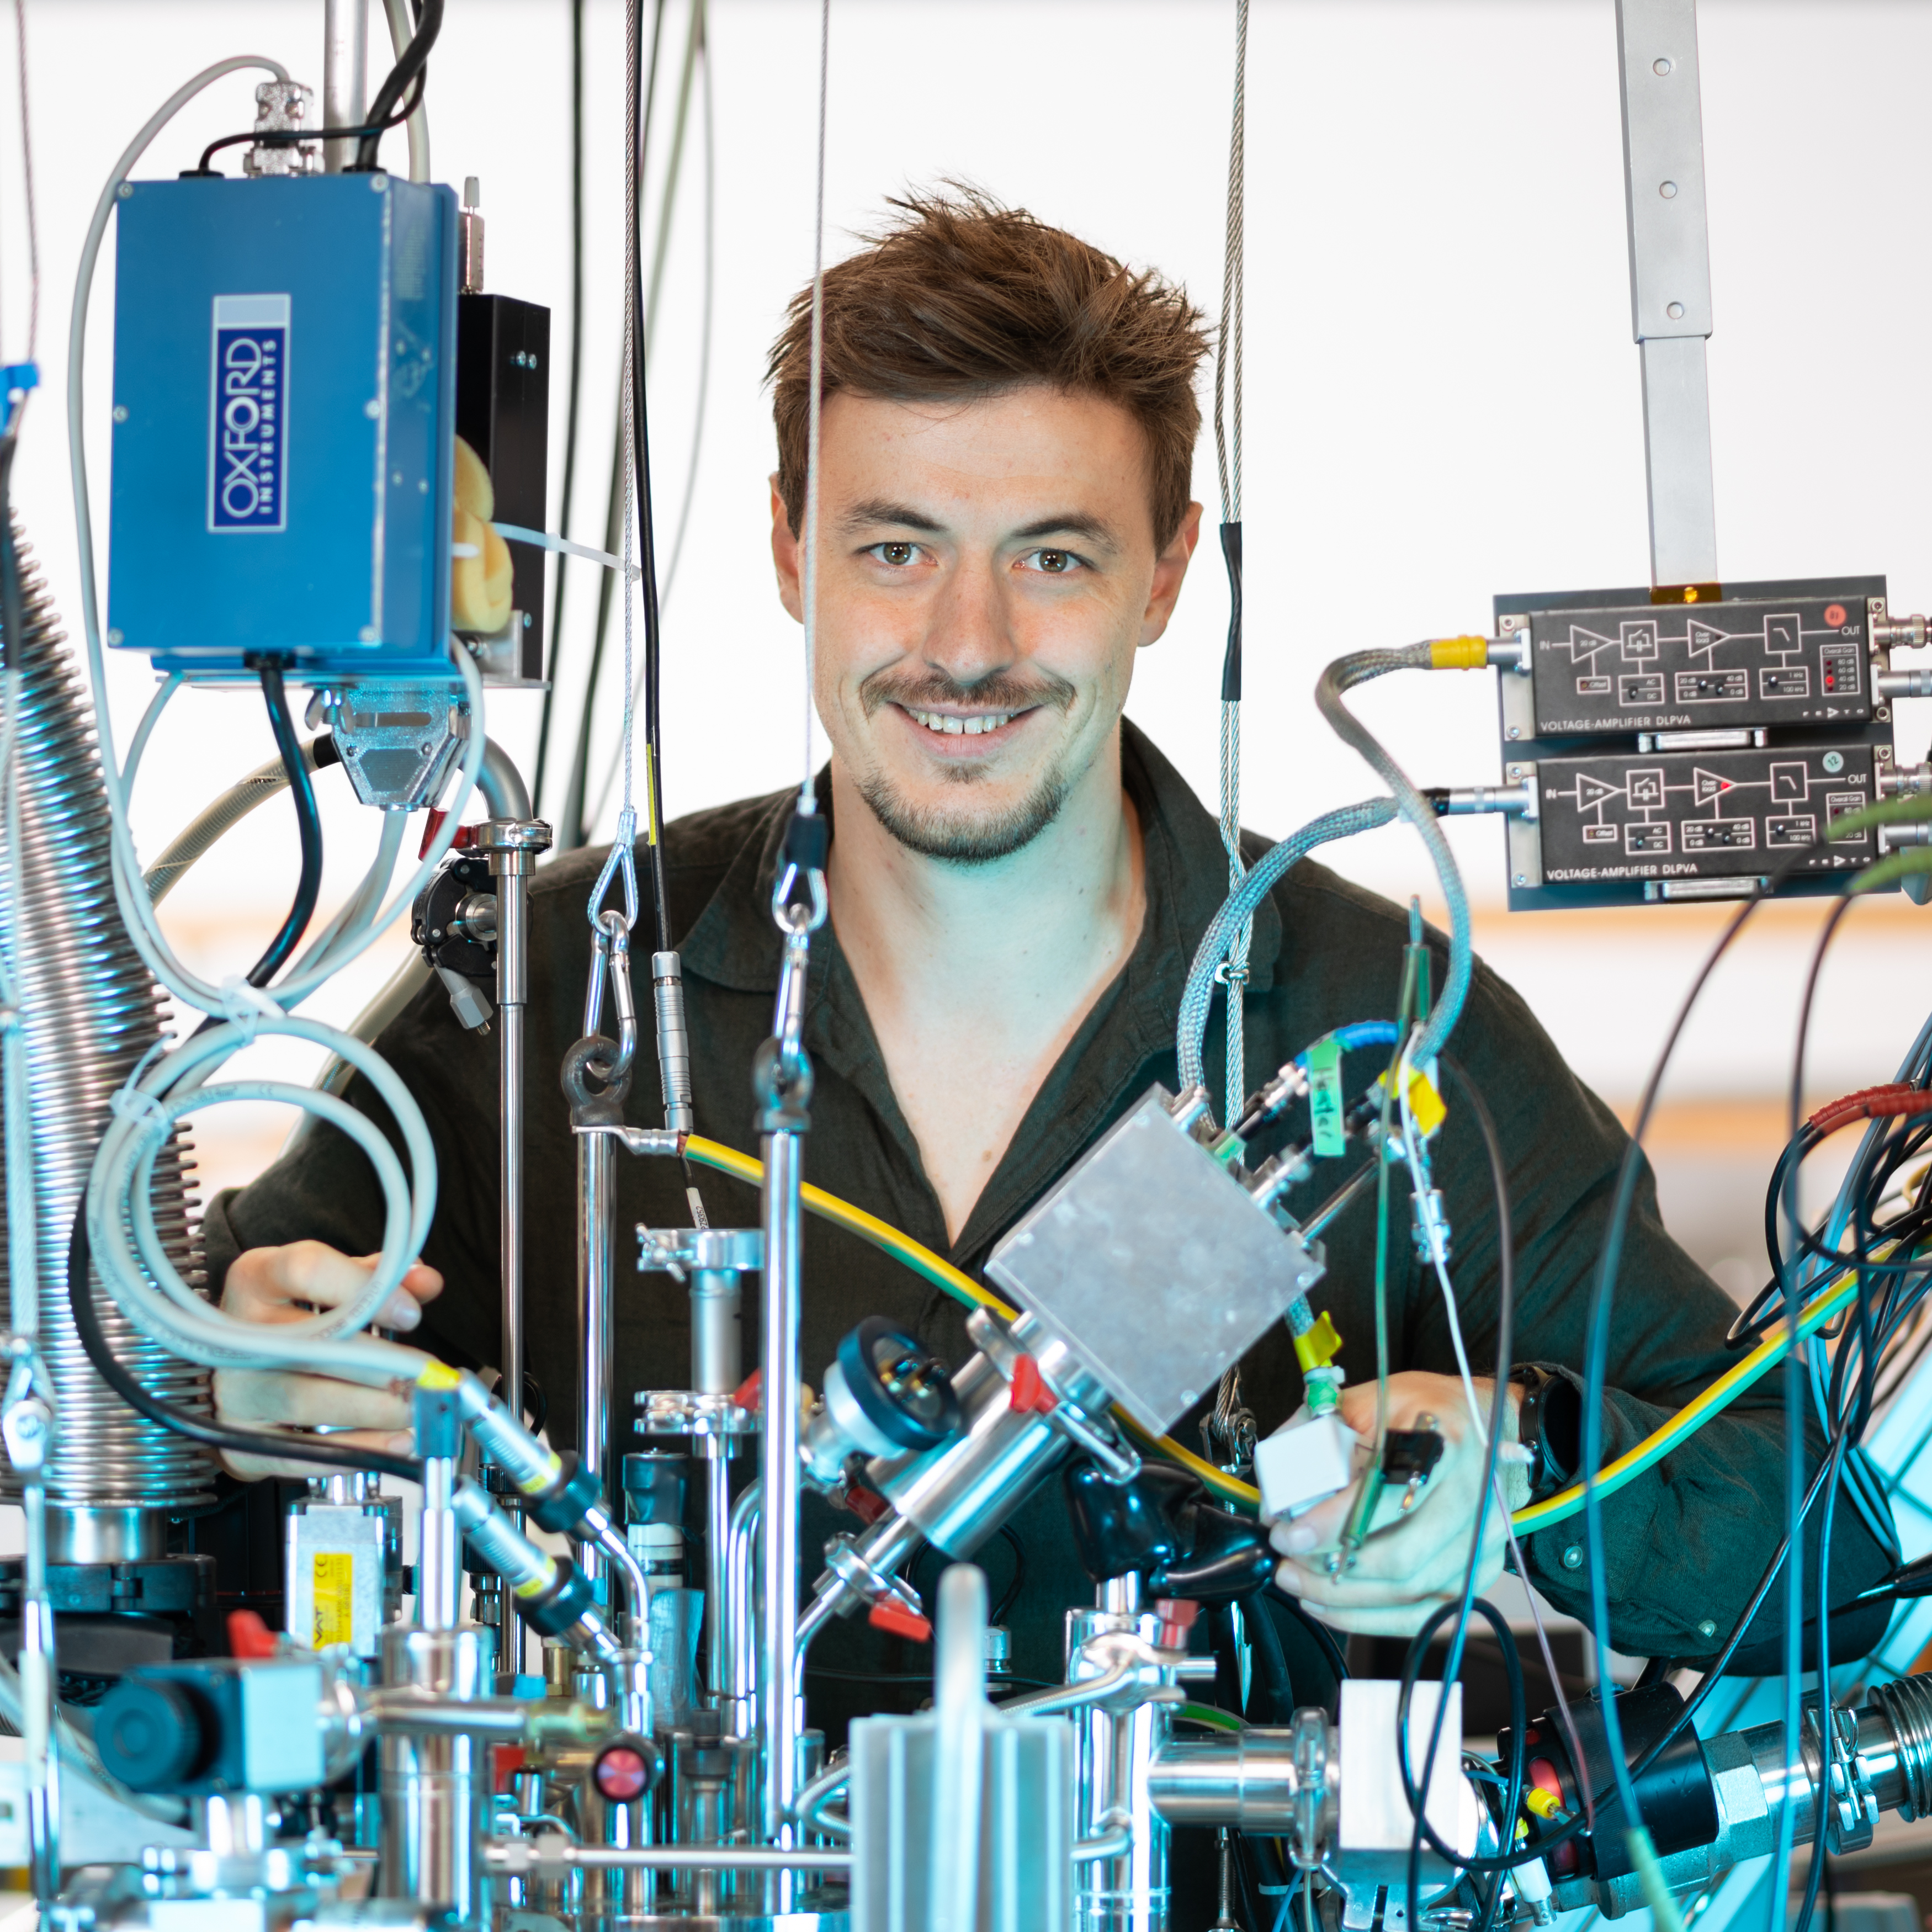
\includegraphics[width=4cm]{miscellaneous/backcover/portrait.jpg}%
    \end{textblock*}%

    \begin{textblock*}{8.3cm}(5.5cm, 8.5cm)%
        \selectfontsize{9pt}%
        \setstretch{1.15}%
        \noindent%
        Oliver Aschenbrenner studies quantum transport in mesoscopic superconducting devices. In the group of Prof.~Dr.~Elke Scheer at the University of Konstanz, he investigates microwave driven transport from tunnel junctions to atomic contacts. His work combines low-temperature experiments, nanofabrication, automated measurements, and quantitative transport models. He earned his bachelor's and master's degrees in physics at the University of Konstanz and gained research experience at Umeå University and the University of Zagreb.%
    \end{textblock*}%
\end{sffamily}%
